\section{Prædiktiv model} \label{prae_model}
\noindent
Til at estimere indlæggelsesvarigheden for patienter kan en prædiktiv model anvendes. 
Prædiktiv modellering er en model, der udarbejdes med henblik på at forudsige hændelser. Denne model skal gøre det muligt at forstå og kvantificere nøjagtigheden af forudsigelsen ift. fremtidig data.\cite{Kuhn2013} Kvantificeringen sker på baggrund af algoritmer. 


Inden for sundhedssektoren er det muligt at prædiktere forskellige former for hændelser og forløb. Dette kan eksempelvis være en forudsigelse om, hvorvidt en patient, indlagt med hjertestop, har risiko for endnu et hjertestop, hvoraf vurderingen f.eks. baseres på demografi, livsstil samt kliniske målinger\cite{Hastie2008}.  \\

\noindent
Prædiktiv modellering kan opdeles i de to kategorier: parametrisk og ikke-parametrisk. Parametrisk anvendes, når samtlige parametre er kendte, hvorimod ikke-parametriske benyttes, hvis én eller flere er ukendte.\cite{Sheskin2000} %Da flere af parametrene i datasættet ikke er kendte bør der anvendes ikke-parametrisk modellering.\cite{Sheskin2000}


Den prædiktive model kan både anvende matematiske- og computerbaserede modeller. Matematiske modeller er en ligningsbaseret model, der forudsiger på baggrund af ændring i input. Herunder anvendes ofte regression, hvor der tages udgangspunkt i lineær sammenhæng. Computerbaserede modeller kræver ofte en simuleringsteknik til forudsigelse.\cite{MathWorks2016}


Som tidligere nævnt sker kvantificering ud fra algoritmer. For at kunne udarbejde en algoritme kræves et træningssæt\cite{DIKU2010}. Et træningssæt kan både være supervised eller unsupervised. Supervised learning er når indholdet af datasamples har til formål at forudsige en hændelse på baggrund af den kendte input-output relation\cite{Brownlee2013}. Modsat er unsupervised learning, når indholdet af datasamples ikke har til formål at prædiktere en hændelse, men derimod finde en sammenhæng mellem data\cite{Brownlee2013, Kuhn2013}. %Datasættet fra ortopædkirurgisk afdeling på Aalborg Universitetshospital indeholder både input-output relation, hvorfor der bør benyttes supervised learning. 
På baggrund af ovenstående er \figref{praediktiv} udarbejdet. Denne illustrerer de valg, der burde tages ift. prædiktive modeller.

\begin{figure}[H]
	%\flushleft 
	\centering
	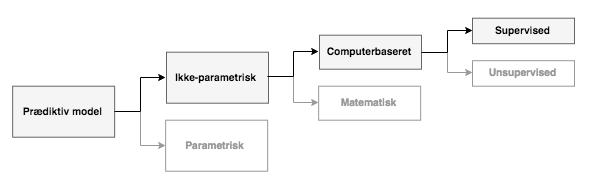
\includegraphics[scale=.73]{figures/praediktivmodel.png}
	%\flushleft
	\caption{\textit{Valg ift. prædiktiv modellering. De markerede felter illustrerer beslutningstagen.}}
	\label{praediktiv}
\end{figure}

\noindent 
Det fremgår af \figref{praediktiv}, hvilke modeller, der bør anvendes ud fra datasættet fra ortopædkirurgisk afdeling.
Da flere af parametrene i datasættet ikke fremgår bør der anvendes ikke-parametrisk modellering. Datasættet består af flere parametre, hvilket medfører, at det ikke ses hensigtmæssigt at anvende ligningsbaseret modellering. Hertil kræves en simuleringsteknik, der anvendes under computerbaseret modellering. Der afgrænses til supervised learning, da datasættet indeholder input-output relation.


\subsection{Præprocessering}
Da flere parametre i datasættet fra ortopædkirurgisk afdeling på Aalborg Universitetshospital mangler, anses det nødvendigt at foretage præprocessering. Præprocessering foregår manuelt før en prædiktiv modellering kan foretages.
Der findes flere metoder, der kan anvendes for at kompensere for de manglende parametre. Kompenseringen kan forekomme ved kassering af værdier, tilegne manglende værdier, reducering af værdier og imputering. Imputering opdeles i tre underkategorier: Prædiktiv værdi imputation, Distribution-baserede imputation og Unik-værdi imputation. Prædiktiv værdi imputation erstatter den manglende værdi med estimerede værdier. Distribution-baserede imputation vægter værdien af manglende data mindre end det resterende, således disse får en mindre betydning under generering. Unik-værdi imputation  erstatter den manglede værdi med en vilkårlig værdi fra samme parameter.\cite{Saar2007} 


